\documentclass[tikz,border=10pt]{standalone}
\usetikzlibrary{shapes.geometric, arrows.meta, positioning, calc}

\begin{document}
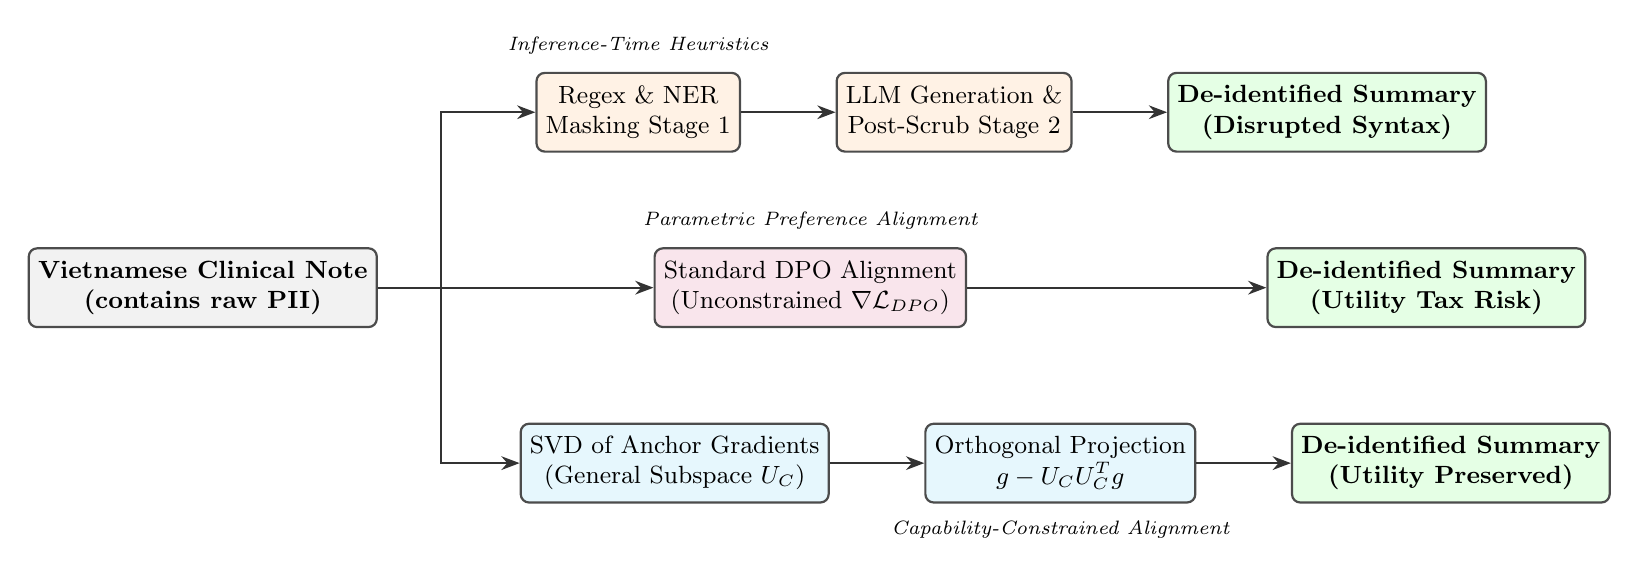
\begin{tikzpicture}[
    node distance=1.5cm and 1.8cm,
    box/.style={
        rectangle, 
        draw=black!70, 
        fill=blue!5, 
        thick, 
        rounded corners=3pt, 
        align=center, 
        minimum height=1.0cm, 
        minimum width=2.5cm,
        font=\small
    },
    inputbox/.style={
        box, 
        fill=gray!10, 
        minimum width=3.2cm,
        font=\small\bfseries
    },
    outputbox/.style={
        box, 
        fill=green!10, 
        minimum width=3.0cm,
        font=\small\bfseries
    },
    filterbox/.style={
        box, 
        fill=orange!10
    },
    dpobox/.style={
        box, 
        fill=purple!10
    },
    ogpsabox/.style={
        box, 
        fill=cyan!10
    },
    arrow/.style={
        -{Stealth[scale=1.0]}, 
        thick, 
        draw=black!80
    },
    labelstyle/.style={
        font=\scriptsize\itshape,
        align=center
    }
]

    % Input
    \node[inputbox] (input) {Vietnamese Clinical Note\\(contains raw PII)};

    % Path 1: Privacy Filter (Top)
    \node[filterbox, above right=1.2cm and 2.0cm of input] (pf_ner) {Regex \& NER\\Masking Stage 1};
    \node[filterbox, right=1.2cm of pf_ner] (pf_gen) {LLM Generation \&\\Post-Scrub Stage 2};
    \node[outputbox, right=1.2cm of pf_gen] (pf_out) {De-identified Summary\\(Disrupted Syntax)};

    % Path 2: Standard DPO (Middle)
    \node[dpobox, right=3.5cm of input] (std_dpo) {Standard DPO Alignment\\(Unconstrained $\nabla \mathcal{L}_{\text{DPO}}$)};
    \node[outputbox, right=3.8cm of std_dpo] (dpo_out) {De-identified Summary\\(Utility Tax Risk)};

    % Path 3: OGPSA-DPO (Bottom)
    \node[ogpsabox, below right=1.2cm and 1.8cm of input] (ogpsa_svd) {SVD of Anchor Gradients\\(General Subspace $U_C$)};
    \node[ogpsabox, right=1.2cm of ogpsa_svd] (ogpsa_proj) {Orthogonal Projection\\$g - U_C U_C^T g$};
    \node[outputbox, right=1.2cm of ogpsa_proj] (ogpsa_out) {De-identified Summary\\(Utility Preserved)};

    % Branching paths from Input
    \draw[arrow] (input.east) -- +(0.8,0) |- (pf_ner.west);
    \draw[arrow] (input.east) -- (std_dpo.west);
    \draw[arrow] (input.east) -- +(0.8,0) |- (ogpsa_svd.west);

    % Path 1 Flows
    \draw[arrow] (pf_ner) -- (pf_gen);
    \draw[arrow] (pf_gen) -- (pf_out);

    % Path 2 Flows
    \draw[arrow] (std_dpo) -- (dpo_out);

    % Path 3 Flows
    \draw[arrow] (ogpsa_svd) -- (ogpsa_proj);
    \draw[arrow] (ogpsa_proj) -- (ogpsa_out);

    % Legend / Labels
    \node[labelstyle, above=0.1cm of pf_ner] {Inference-Time Heuristics};
    \node[labelstyle, above=0.1cm of std_dpo] {Parametric Preference Alignment};
    \node[labelstyle, below=0.1cm of ogpsa_proj] {Capability-Constrained Alignment};

\end{tikzpicture}
\end{document}
